% Copyright (c) 2014,2016,2018 Casper Ti. Vector
% Public domain.

\chapter{引言}
%\pkuthssffaq % 中文测试文字。

\section{云计算的基本概念}

云计算(Cloud Computing),根据美国国家标准技术研究所(NIST)的定义,指的是一种可以实现对可配置计算资源共享池(如网络、服务器、存储、应用和服务)进行随时随地、便捷、按需网络访问模型。这些资源可以迅速地配分配和释放,并且这个过程只需要足最低限度的资源管理工作以及与服务提供商最少的交互。美国亚马逊公司再2006年3月推出了 Amanzon Web Service(AWS),这一事件一般被认为代表着云计算时代的正式开启。经过十几年的发展,凭借着“方便易用、弹性伸缩、按需服务”的技术特征,云计算概念已被广泛接受,云计算产业取得了商业上的巨大成功,云计算平台已成为当今社会的关键信息基础设施,云计算技术为大数据、人工智能的领域的蓬勃发展特工了重要的支撑作用。

\subsection{云计算的传统服务模型}

NIST 将云计算分为了三种服务模型。

这三种服务模型分别是基础设施即服务(Infrastructure as a Service,IaaS)、平台即服务(Platform as a Service,PaaS)以及软件即服务(Software as a Service,SaaS)。IaaS为消费者提供用来运行应用的计算资源,包括服务器、存储、网络等。其中虚拟机是云厂商提供的最核心的IaaS产品。与IaaS只提供最基础的底层资源不同,PaaS强调为消费者提供云开发环境,除计算资源意外,PaaS为用户提供中间件开发,运行平台及工具,帮助用户更方便地开、管理、测试和运行应用。SaaS是厂商提供的基于云的软件,用户无需下载安装软件,通过浏览器即可访问服务。

图\ref{rep_products}给出了云计算三种服务模型的代表产品。亚马逊公司的AWS EC2,谷歌公司的Google Compute Engine以及阿里云公司的ECS都是典型的IaaS产品。其主要服务形态是云厂商向消费者售卖虚拟机或者裸金属服务器以及连带的网络、存储等附属产品。PaaS的代表性产品包括AWS Beanstalk、Google App Engine、Microsoft Azure App Servics等。此类韩品为用户提供再云中快速部署和管理应用的能力,提供包括应用扩容,负载均衡,应用监控和安全管理等功能。相比于IaaS仅售卖以虚拟机为主的基础设施,PaaS降低了用户开发、管理、运维应用的成本,使得用户可以更加专注于构建应用本身。在云计算已经发展了十几年的当今时代,越来越多的SaaS产品涌现了出来。谷歌公司开发的Google Docs、Google Maps以及微软公司开发的Microsoft Office 365都是典型的SaaS产品。以Google Docs为例,与传统的文件处理办公软降相比,用户无需在本地花费大量存储空间来安装软件,只需要打开浏览器,输入URL,即可使用Google Docs服务处理文件,并且所有的文件都会被及时同步保存到云端。另一个代表性的SaaS产品是Google Maps。Google Maps与Google Docs类似,为个人用户提供在浏览器中直接使用的地图服务。与传统软件相比,SaaS在使用方式上具有方便灵活,跨平台的特性,同时用户存储在云端的数据经过云厂商的冗余备份也具有更高的可靠性。

\begin{figure}
    \centerline{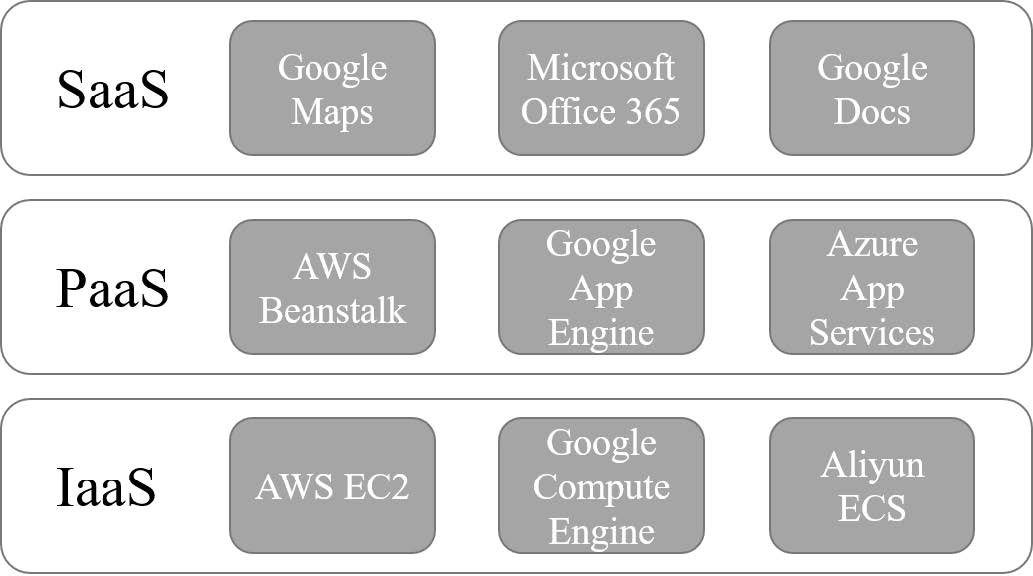
\includegraphics[width=\textwidth]{figures/rep_products.jpg}}
    \caption{云计算服务模型代表产品}
    \label{rep_products}
\end{figure}

\subsection{云计算的新兴服务模型}

云计算发展至今日,其服务模型已经不严格局限于NIST最初总结的这三种基本形态,世界各地各领域的研究者们已经提出了众多不同的X as a Service,包括Blockchain as a Service,Sensing as a Service,Workspace as a Service等。与传统的三种服务形态相比,这些服务不单纯是硬件服务或者软件服务,其结合二者的特点,面向特定的领域方向进行更深度的定制,如区块链、物联网、分布式共识等。服务形态的日益丰富,服务内容的日益复杂体现了云计算更见领域化,精细化的发展趋势。而近几年来最热门的概念莫过于FaaS,即Fucntion as a Service。

FaaS是一种新兴的计算模式,亦被称为Serverless Computing。从字面理解,Serverless Computing即为“无服务器计算”之意。然后,其并非意味着真的没有服务器,而已说开发者不用过多考虑服务器的相关问题。在传统的IaaS服务中,开发者需要自己惊醒服务器管理与运维,负责服务的发布,在流量变化时对服务器集群进行扩容或缩容。而在FaaS中,开发者只需要关注业务逻辑,至于服务的发布、管理、弹性伸缩等,则交由云厂商来完成。

FaaS背后的机制一般是以容器技术为基础的。典型地,开发者上传自己的业务代码后,云厂商并不会直接收费。当对该服务的请求到来之时,云厂商将启动一系列容器来运行该服务,从而对用户的请求进行响应。通常而言,开发者指定的服务会与某些时间绑定(hook),在发生该事件时,立即触发开发者定义的服务。我们以AWS的serverless computing服务Lambda中的一个示例程序为例,讲述整个流程。图\ref{aws_resize}所示的是一个为照片调整大小的服务。该服务与AWS S3(AWS的对象存储服务)的上传事件绑定,当云厂商检测到有用户向S3上传图片时,会立即触发开发者定义的图片大小调整函数。整个流程中,开发者需要关注的只有第四步的函数开发工作,至于该函数的横向拓展,全部由云厂商来负责。

\begin{figure}
    \centerline{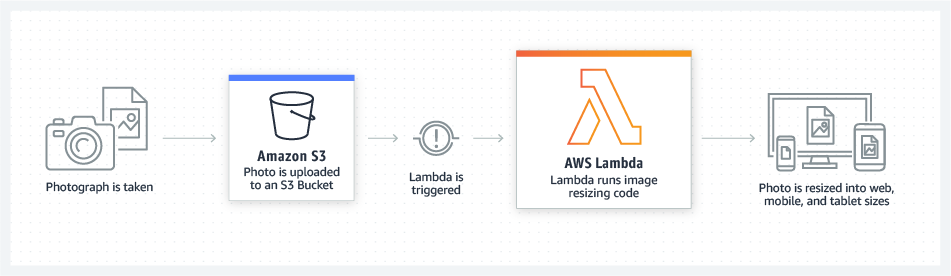
\includegraphics[width=\textwidth]{figures/aws-lambda-resize.png}}
    \caption{AWS Lambda中示例程序:照片大小调整}
    \label{aws_resize}
\end{figure}

主流的云厂商均提供了FaaS服务,例如AWS的Lambda,阿里云的函数计算等,近年来越来越受到开发者的青睐。一方面是因为它的高弹性,易于开发。另一方面则是因为其细粒度的收费模式。通常而言,FaaS的服务是按照请求次数进行收费。当函数闲置时,并不产生额外的费用。

\section{人工智能技术近年的发展}
TODO: 简介近些年人工智能技术的发展

\section{云计算和人工智能交叉领域的常见研究问题}
云计算和人工智能是两个息息相关的热门领域。一方面,以深度学习为典型代表的人工智能技术在当今社会被应用的越来月广泛,研发、调试、发布新的模型的需求日益增长。与这种发展趋势对应,多数主流的云厂商都提供了机器学习模型训练-测试-部署的pipeline。学术界也不断探索“云上机器学习”这一话题,利用新的计算模式(如FaaS)在云上以更便捷、更经济高效地开展ML模型的训练和部署。同时得益于近年硬件技术的发展,多种新硬件(多体现为人工智能的加速芯片)在云环境中得到应用,进一步方便机器学习用户将整个开发流程迁移到云端。另一方面,机器学习技术也越来越多被用于解决云计算中常见的问题。例如使用推荐算法解决置优化问题和利用强化学习解云环境中的资源调度问题。下文对这几个常见问题做简单概述,具体研究将在后续几章展开。

\subsection{基于公有云服务的机器学习平台}
\textbf{1. 产业界}

主流的云厂商都提供了面向机器学习的平台系统,例如AWS和Sagamaker\parencite{joshi2020amazon,liberty2020elastic,perrone2020amazon},Azure的Azure ML Studio\parencite{etaati2019azure}等。这些基于云的平台提供了一站式调试、训练和部署ML模型的能力。一般而言此类平台被视为SaaS类的服务,因为其是基于云资源构建的上层软件栈,使得用户能够直接使用web的方式使用。例如Sagemaker就支持用户直接在浏览器中用jupyter notebook编写和调试模型代码。

\textbf{2. 学术界}

一般而言,产业界的平台系统面向的是一般性用户的普遍需求。因此,对于有特殊需求的用户,通常会有与产业界的解决方案并行的工作。例如,为了以尽可能低的成本在云上完成模型的训练,相关工作\parencite{harlap2017proteus,li2020spottune}尝试利用云上的动态资源(价格低但是稳定性/可用性低)进行模型的训练,并辅以一定的策略增强其可靠性。再比如,机器学习模型的在线服务会有低延迟、高吞吐率的要求。为了实现上述需求,相关工作\parencite{zhang2019mark}利用云上的多种资源(如IaaS,FaaS等),根据负载的动态变化,敏捷地在不同资源之间切换,充分利用不同类型资源的优点,规避掉其缺点,实现高效、经济的模型在线服务。一般而言,学术界的此类研究构建于云厂商服务的上层,是一种Cloud-of-Clouds的模式。

\subsection{利用新的计算模式在云上运行机器学习pipeline}
以FaaS为代表的新型云计算模式,以其高弹性、灵活的计费方式等特点吸引了众多研究者的注意。学术界开始探讨如何使得机器学习工作流享用到FaaS的诸多优点。


\subsection{面向人工智能的专用芯片}
\subsection{利用机器学习算法解决配置优化问题}
\subsection{利用机器学习算法解决资源调度问题}
% vim:ts=4:sw=4
